% !TeX spellcheck = en_US
\chapter{Results}

For the large set of simulations we can now extract the needed values. The output of the relaxation program (\texttt{spheres\_ini\_log}) gives us the precise values for impact angle and velocity and the exact masses of all bodies. As these values differ slightly from the parameters explained in Section \ref{sec:parameters} due to the setup of the simulation, in the following steps only the precise values are considered. From the \texttt{aggregates.txt} explained in Section \ref{sec:postprocessing} the final masses and water fractions of the two largest fragments are extracted. From these the main output considered in this analysis, the water retention of the two fragments can be calculated. 

\section{Correlations}
\label{sec:cov}
One very easy, but sometimes flawed%
\footnote{Pearson correlation coefficient only measures linear correlations. With a value close to zero can still be a non-linear correlation between the two dimensions. In addition the coefficient gives no information about the steepness of the correlation, only about which fraction of the values conform to it.} 
way to look at the whole dataset at once is calculating the \textit{Pearson correlation coefficient} between the input parameters and the output water fraction (Figure \ref{fig:cov}). This shows the expected result that a higher collision angle (so a more hit-and-run like collision) has a higher water retention and a higher collision speed results in less water left on the two largest remaining fragments. In addition, higher masses seem to result in less water retention. The initial water fractions of the two bodies does seem to have very little influence on the result of the simulations.

\begin{figure}
	\centering
	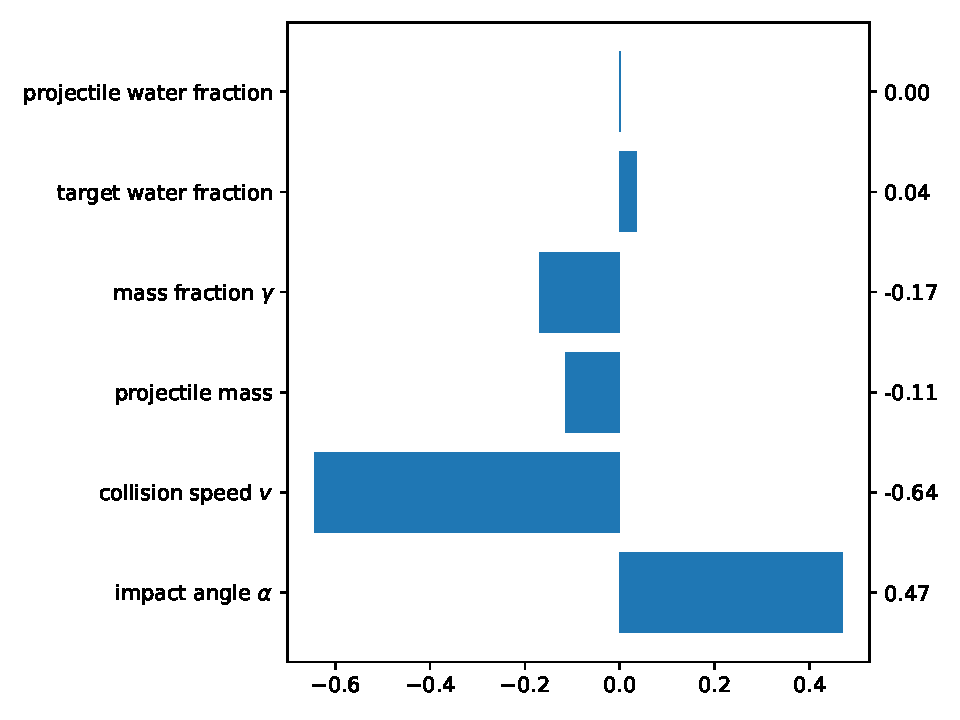
\includegraphics[width=0.8\linewidth]{images/cov.pdf}
	\caption{TODO}
	\label{fig:cov}
\end{figure}